

\documentclass[12pt]{article}
\usepackage{fullpage,threeparttable,harvard,threeparttable,endnotes,setspace,amsmath,amssymb,rotating}
\usepackage{amsmath,amssymb}

\newtheorem{assump}{Assumption}
\newtheorem{hyp}{Hypothesis}
\newtheorem{hunch}{Proposition}
\newtheorem{impl}{Implication}
 
\voffset=-1mm
 
\begin{document}

\vspace{50mm}


\title{An Analysis of Some Rather Arbitrary Stuff: Illustrating \LaTeX~  basics\thanks{Thanks to all those who made this possible, but shouldn't have.}}
 
\author{Me \and Myself \and I }

\maketitle \thispagestyle{empty}

\begin{abstract}

This abstract is the short version of the much longer version below.  The longer version below is longer than this shorter version. This shorter version, though, is still longer than it needs to be, but not as much longer-than-it-needs-to-be as the longer version that follows.

\end{abstract}
 \clearpage


\pagebreak
\thispagestyle{empty} \clearpage \pagebreak \pagestyle{plain}  \doublespace

This is where the paper begins, with a beginning, outlining what I will try to persuade the reader to believe. In this paper, I will explore randomly typed numbers. Some scholars hold that randomly typed numbers hold little significance in terms of understanding causal processes \cite{dover1999insignificance}. Others, on the other hand, suggest the sources of randomness are hardly random, but derive from keen interest in brewed or fermented spirits \cite{adams1766brewing}. The careful reader will also notice the paper illustrates a large number of basic features of \LaTeX. \cite{binmore85}

\section*{The Next Section}
 
 Some math: suppose two matrices as follows: 
 
$$\left[\begin{array}{ccc}1 & 2 & 3 \\4 & 5 & 6 \\2 & 4 & 9\end{array}\right]   \left(\begin{array}{c}1 \\1 \\1\end{array}\right)$$ 

and a model like this:
 
\begin{eqnarray}
ln \text{L} = \sum\limits_{i=1}^{n} -\left(\frac{z_1\gamma_1}{2}\right) - \left(\frac{z_2\gamma_2}{2}\right) - \left(\frac{ln(1-\rho^2)}{2}\right) - \frac{1}{2(1-\rho^2)}   \nonumber \\ \nonumber \\
\left[ \frac{(y_1-x_1\beta_1)^2}{e^{z_1\gamma_1}} - 2\rho\frac{(y_1-x_1\beta_1)(y_2-x_2\beta_2)}{e^{\left(\frac{z_1\gamma_1}{2}\right)} e^{\left(\frac{z_2\gamma_2}{2}\right)}} +   \frac{(y_2-x_2\beta_2)^2}{e^{(z_1\gamma_1)}}\right] \nonumber
\end{eqnarray}

This is a long equation meant to illustrate a number of things. One might also want ``in-line'' math which means math in the line of the text (rather than off-set as the equation above. Accomplishing that is simple: the error in the model described above is $\epsilon \sim N_{2} (\beta_{1,2}, \sigma^{2}_{1,2}, \rho_{1,2})$. 


  
\section*{Good Grief, Another Section}
Yet more words still.

\subsection*{A Subsection, no less}
More words hopefully related to the theme of the section. The foregoing discussion leads to the following hypotheses:

\begin{hyp}
If I randomly type numbers in a table, the numbers in the table will be random.
\end{hyp}

Further, it follows that: 

\begin{hyp}
A figure of randomly chosen numbers will be just as meaningless as a table of those same numbers.
\end{hyp}

Evaluating these hypotheses requires unique data. I will generate appropriate data using the ``{\sf gennorm}'' feature in ``{\sf Stata}.''\footnote{While it is true I am making up the data, I am doing so with the highest sort of principles. To make sure the random data are random, I replicated this process using ``{\sf generate double z = runiform()} and achieved the same results. }

\subsection*{Another Subsection, believe it or not}

This subsection contains a list:

\begin{itemize}
\item This is the {\bf first} thing on the list.
\item This is the {\it second} thing on the list.
\end{itemize}


\section*{Another Section because damn, this is a long paper}

This section has a table in it. It uses the ``{\sf threeparttable.sty}'' style, those three parts being a caption, the body of the table, and table notes explaining what the table contains. 

\begin{table}[ht]
\begin{center}
\begin{threeparttable}
\caption{A Table of Some Numbers I Made Up\tnote{\dag}} \label{tab:somenumbers}
\begin{tabular}{lrrr}
\hline \hline
 &Coefficient  &Std. Err. & z-score\\ \hline

%&\multicolumn{2}{c}{WEIS, 1966-1992}			~		& \multicolumn{2}{c}{COPDAB, 1948-1979}		 \\ \hline

Meaningful Variable 1	&	0.001	&	0.019	&	0.06	\\
Meaningful Variable 2	&	11.525*	&	3.010	&	3.83	\\
Meaningful Variable 3 &	-1.296*	&	0.529	&	-2.45	\\
intercept	&	-2.023*	&	0.143	&	-14.16	\\ \\

N & 3  \\
model $\chi^2$	& 63.53*				\\ \hline

\hline \hline

\end{tabular}
\begin{tablenotes}
\item[\dag] {{\footnotesize These numbers are the numbers I randomly hit on the keyboard. * p $\leq$ .01}}
\end{tablenotes}
\end{threeparttable}
\end{center}
\end{table}


The model estimates in Table \ref{tab:somenumbers} are broadly consistent with my having typed numbers into a table. This is what my hypotheses anticipated. Figure \ref{fig:apicture} illustrates the strong support for the hypotheses.

\begin{figure}[h!]
\begin{centering}
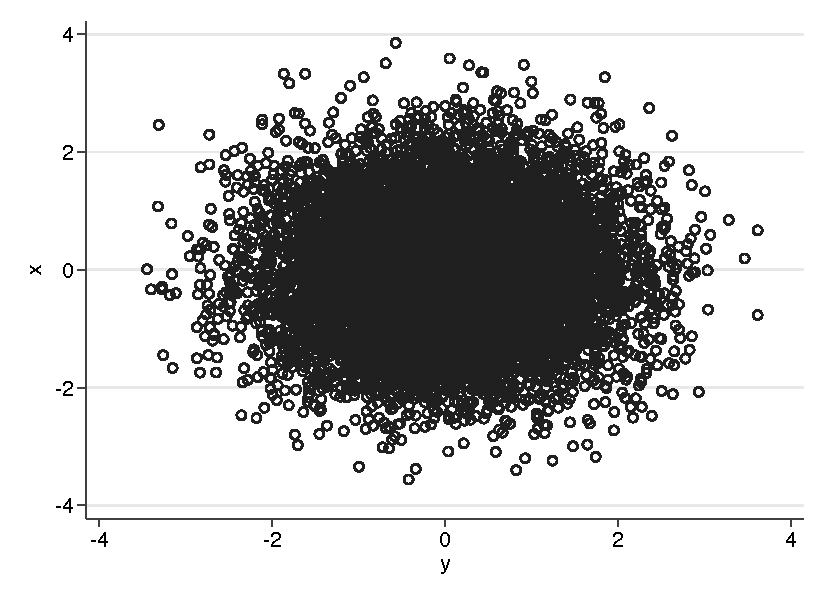
\includegraphics[width=4in]{somenumbers.pdf} 
\caption{The relationship between random typing and numbers in a table.}  \label{fig:apicture}
\end{centering}
\end{figure}


As you can see, randomly generated, uncorrelated numbers are, in fact, unrelated to one another. The pattern in Figure \ref{fig:apicture} is clear evidence two random series are unrelated.

\section*{The Last Section}
 
 This section discusses my findings, namely that random numbers generally seem to lack a pattern. Despite that, it still remains potentially interesting to explore how randomness arises, and if it sometimes might arise due to consumption. As Sam Adams, brewer and patriot, is alleged to have once said, ``brewing is not random, but my cousin John sure as hell is'' \cite{adams1766brewing}.\footnote{I made this up. Completely. It's fake.} Moreover, as the inimitable Colonel Sanders famously said, ``I'm too drunk to taste this chicken'' \cite{ferrell2006talladega}. If that does not prove the point, then it is not clear what will. 
 
 
\clearpage
\pagebreak
\doublespace
\bibliographystyle{polsci}
\bibliography{bibliography}

\end{document}


